% ─── Slide: INT4 PTQ journey ──────────────────────────────────────────────────
\begin{frame}[shrink=20]{INT4 Pure PTQ: A Stepwise Story}
  \begin{columns}[T]
    \begin{column}{0.48\textwidth}
      \textbf{Each step fixes one failure mode:}

      \begin{enumerate}
        \small
        \item \textbf{Baseline INT4 (128 samples):}
          $\adcppl = 2355$ — catastrophic; 128 samples insufficient.

        \item \textbf{Propagation + 1024 samples:}
          $\adcppl = 40.6$ — scale and propagation are the dominant levers.

        \item \textbf{Partial propagation $\alpha = 0.5$:}
          $\adcppl = 31.2$ then \textbf{diag scaling} $\to 27.56$ —
          mixed FP+quant loss + bounded diagonal.

        \item \textbf{Staged training (MLP $\to$ attn diag):}
          $\adcppl = 27.60$, $\no-ADC = 18.50$ — cleanest no-ADC yet.
      \end{enumerate}

      \vspace{0.15em}
      \begin{alertblock}{Key insight}
        Bin-centre loss is \worse{harmful} for INT4:
        fine ADC step ($\delta{\approx}6.12$) makes the penalty
        dominate and destabilise training.
      \end{alertblock}
    \end{column}
    \begin{column}{0.48\textwidth}
      % plot_int4_ptq_progression.pdf
      \iftrue
        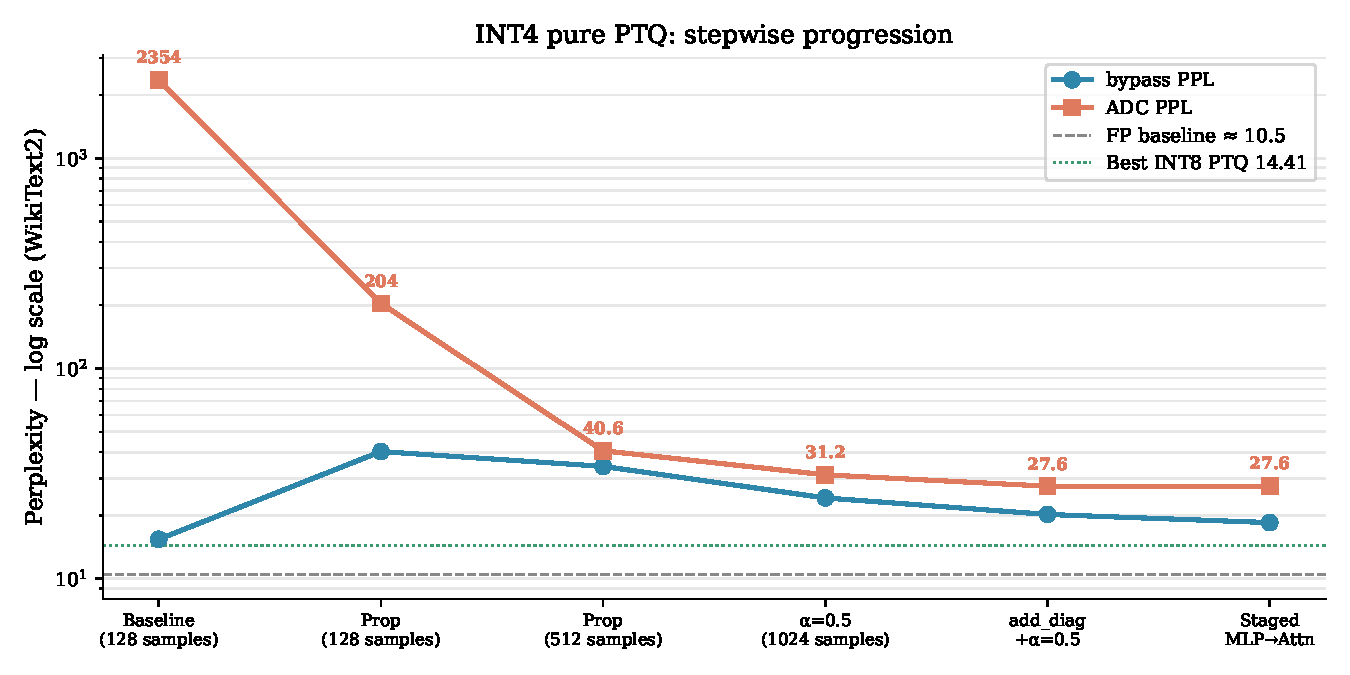
\includegraphics[width=\linewidth]{figs/plot_int4_ptq_progression.pdf}
      \else
        \figplaceholder[0.70\textheight]{Step plot (x = method index 1--6,
          log y-axis = PPL).
          Two lines: no-ADC PPL (blue) and ADC PPL (orange).
          Annotate each step with the key change.
          Show FP baseline as dashed line at 10.5 and INT8-prop+center at 14.41.
          Key numbers: 2355, 204, 40.6, 31.2, 27.56, 27.60.}
      \fi
    \end{column}
  \end{columns}
\end{frame}
